\newpage
\section{Rowcrosser} %\makebox[\linewidth]{\rule{\textwidth}{0.4pt}
{\bf Designer: } Martin Wearn\\
{\bf Cell Description: } A row crossing cell.\\
\subsection*{Dimensions}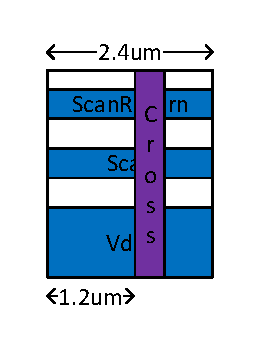
\includegraphics[width=\textwidth,height=4cm,keepaspectratio=true]{../rowcrosser/blackbox.pdf}

\section{Tie High} %\makebox[\linewidth]{\rule{\textwidth}{0.4pt}
{\bf Designer: } Martin Wearn\\
{\bf Cell Description: } A tie to Vdd cell.\\
\subsection*{Dimensions}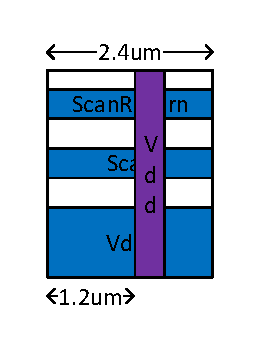
\includegraphics[width=\textwidth,height=4cm,keepaspectratio=true]{../tiehigh/blackbox.pdf}

\section{Tie Low} %\makebox[\linewidth]{\rule{\textwidth}{0.4pt}
{\bf Designer: } Martin Wearn\\
{\bf Cell Description: } A  tie low cell.\\
\subsection*{Dimensions}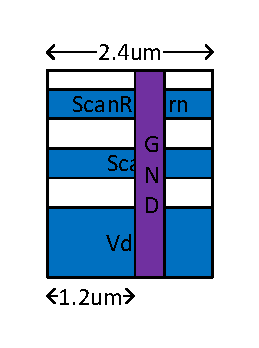
\includegraphics[width=\textwidth,height=4cm,keepaspectratio=true]{../tielow/blackbox.pdf}